\section{meshmorph.cc File Reference}
\label{meshmorph_8cc}\index{meshmorph.cc@{meshmorph.cc}}
{\tt \#include \char`\"{}meshmorph.h\char`\"{}}\par
{\tt \#include $<$iostream$>$}\par
{\tt \#include $<$cassert$>$}\par
{\tt \#include $<$cmath$>$}\par
{\tt \#include \char`\"{}log.h\char`\"{}}\par
{\tt \#include \char`\"{}nice.h\char`\"{}}\par
{\tt \#include \char`\"{}energy.h\char`\"{}}\par
{\tt \#include \char`\"{}controls.h\char`\"{}}\par
{\tt \#include \char`\"{}container.h\char`\"{}}\par
{\tt \#include \char`\"{}refractory.h\char`\"{}}\par
{\tt \#include \char`\"{}virtual\_\-disp.h\char`\"{}}\par
{\tt \#include \char`\"{}gain\_\-schedule.h\char`\"{}}\par
{\tt \#include \char`\"{}vertex\_\-schedule.h\char`\"{}}\par
{\tt \#include \char`\"{}octree\_\-agent\_\-face.h\char`\"{}}\par
{\tt \#include \char`\"{}intersecting\_\-faces.h\char`\"{}}\par
{\tt \#include \char`\"{}octree\_\-visitor\_\-face.h\char`\"{}}\par


Include dependency graph for meshmorph.cc:\begin{figure}[H]
\begin{center}
\leavevmode
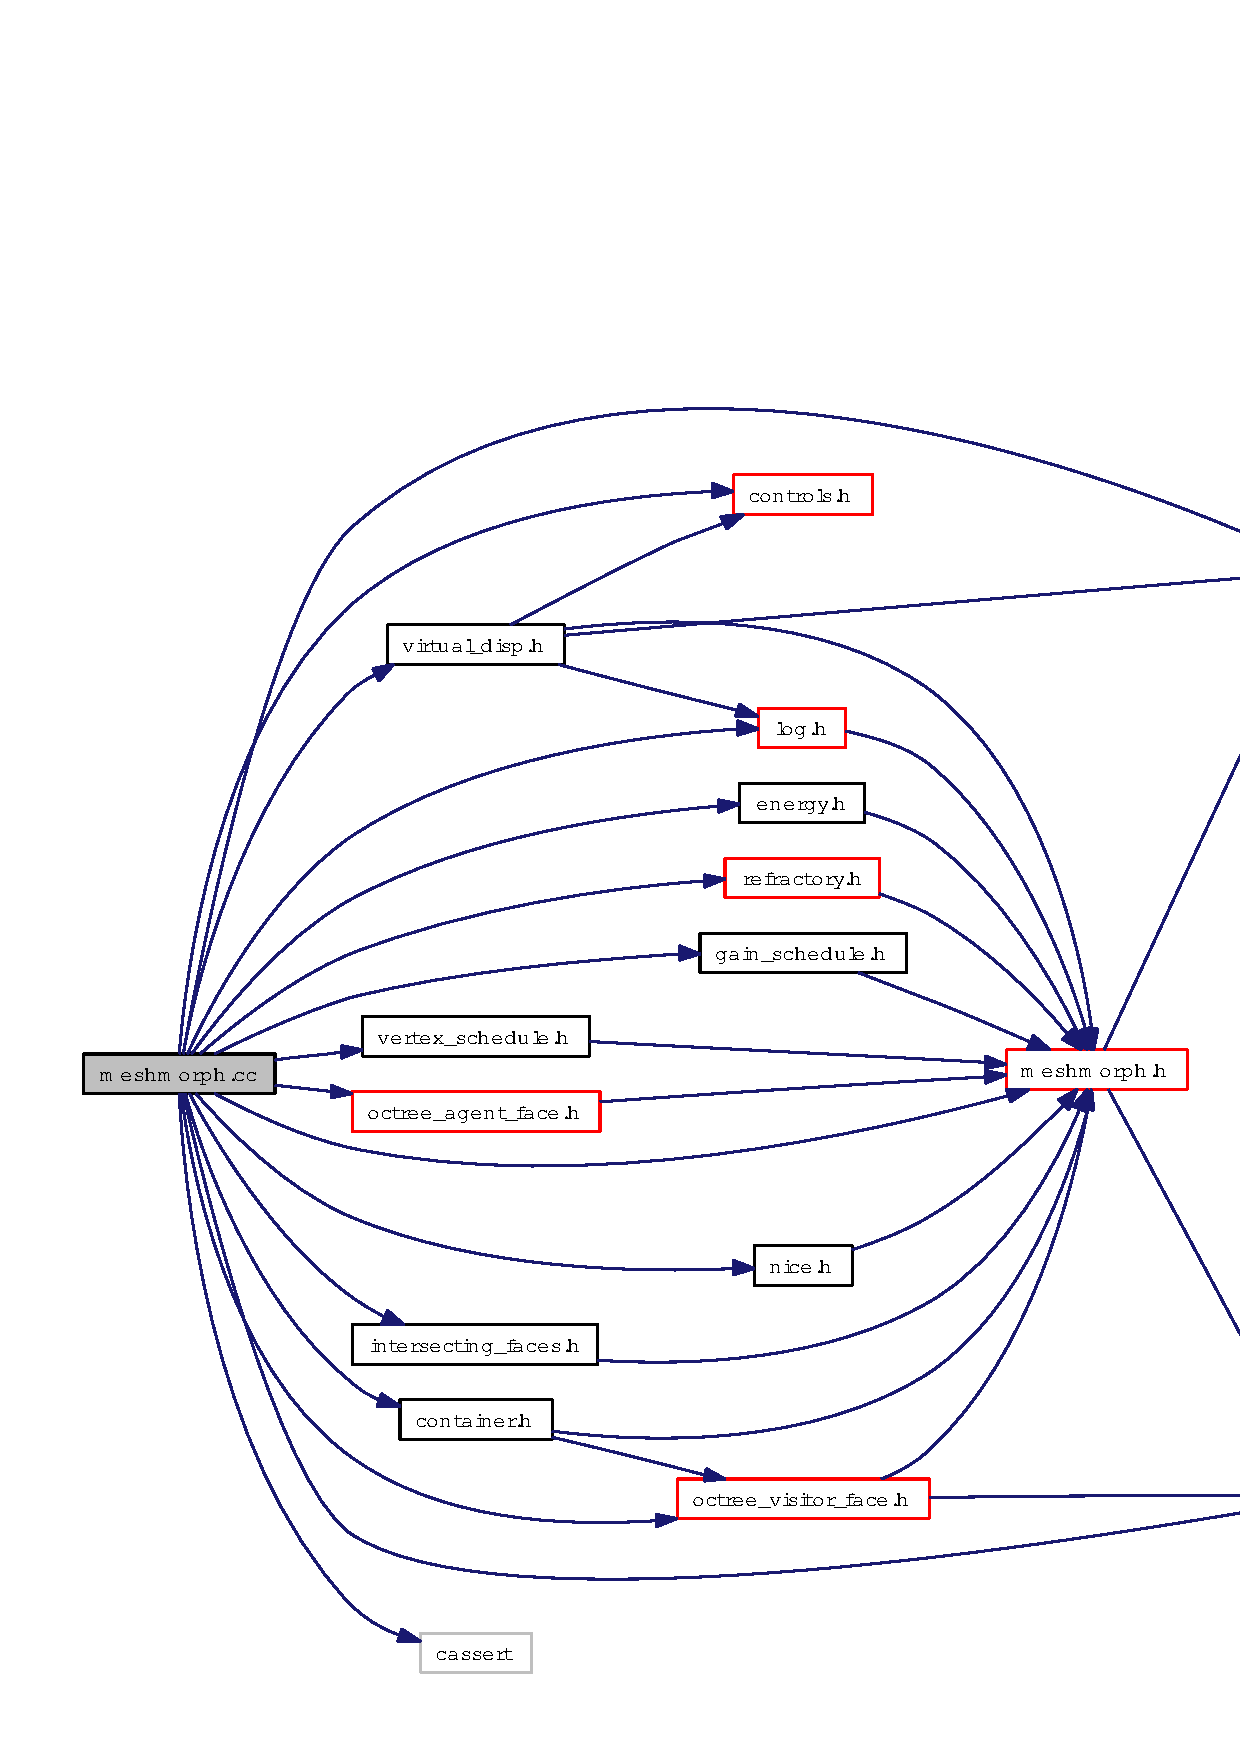
\includegraphics[width=336pt]{meshmorph_8cc__incl}
\end{center}
\end{figure}
\subsection*{Functions}
\begin{CompactItemize}
\item 
int {\bf main} (int argc, char $\ast$$\ast$argv)
\item 
bool {\bf check\-Int\-Size} (void)
\item 
bool {\bf distinguishable} (double a, double b, double epsilon)
\item 
bool {\bf distinguishable} (double a, double b)
\end{CompactItemize}


\subsection{Function Documentation}
\index{meshmorph.cc@{meshmorph.cc}!checkIntSize@{checkIntSize}}
\index{checkIntSize@{checkIntSize}!meshmorph.cc@{meshmorph.cc}}
\subsubsection{\setlength{\rightskip}{0pt plus 5cm}bool check\-Int\-Size (void)}\label{meshmorph_8cc_1122d758f1b6eac91f763e9b10d306d2}


Determine if integers are 32 bit. \begin{Desc}
\item[Returns:]True if integers are 32 bit on this machine; false otherwise. \end{Desc}
\index{meshmorph.cc@{meshmorph.cc}!distinguishable@{distinguishable}}
\index{distinguishable@{distinguishable}!meshmorph.cc@{meshmorph.cc}}
\subsubsection{\setlength{\rightskip}{0pt plus 5cm}bool distinguishable (double {\em a}, double {\em b})}\label{meshmorph_8cc_7e48ad73971e78bc20e3deb1e74546ad}


Determine if two floating-point precision numbers are equivalent in value within MY\_\-DOUBLE\_\-EPSILON. \begin{Desc}
\item[Parameters:]
\begin{description}
\item[\mbox{$\leftarrow$} {\em a}]First number. \item[\mbox{$\leftarrow$} {\em b}]Second number. \end{description}
\end{Desc}
\begin{Desc}
\item[Returns:]1 if Inputs are different; 0 otherwise. \end{Desc}
\index{meshmorph.cc@{meshmorph.cc}!distinguishable@{distinguishable}}
\index{distinguishable@{distinguishable}!meshmorph.cc@{meshmorph.cc}}
\subsubsection{\setlength{\rightskip}{0pt plus 5cm}bool distinguishable (double {\em a}, double {\em b}, double {\em epsilon})}\label{meshmorph_8cc_54baf86f92ae2f215fbf2fc9d9913868}


Determine if two floating-point precision numbers are equivalent in value within epsilon. \begin{Desc}
\item[Parameters:]
\begin{description}
\item[\mbox{$\leftarrow$} {\em a}]First number. \item[\mbox{$\leftarrow$} {\em b}]Second number. \item[\mbox{$\leftarrow$} {\em epsilon}]The difference between the two input values must be greater than the fraction of the largest input value defined by epsilon. \end{description}
\end{Desc}
\begin{Desc}
\item[Returns:]1 if Inputs are different; 0 otherwise. \end{Desc}
\index{meshmorph.cc@{meshmorph.cc}!main@{main}}
\index{main@{main}!meshmorph.cc@{meshmorph.cc}}
\subsubsection{\setlength{\rightskip}{0pt plus 5cm}int main (int {\em argc}, char $\ast$$\ast$ {\em argv})}\label{meshmorph_8cc_3c04138a5bfe5d72780bb7e82a18e627}


